\section*{Extra Experiment}
Extra 실험 1, 2는 주어진 Week 08을 이용하여 Topology를 구성해준다. mininet의 Net command를 이용해서, 주어진 python custom topology code를 통해서 week07과포트의 연결은 동일하고 각 링크와 latency에만 변화가 생겼음을 확인할 수 있었다.
Experiment 2,3 에서 확인해본 Statical Routing과 shortest algorithm 기반의 dynamic routing이외에 네트워크를 이용하는 application을 고려하는 application-aware routing을 실험해보고자 한다. 특정 Bandwidth, Latency를 만족시키는 경로를 찾아 statical routing을 통해서 flow table을 만들어주고, 해당 path가 application의 조건을 만족시키는지 확인해 보았다.
Application X는 latency를, Application Y는 bandwidth에 우선순위를 두는 application 이다.
    \vspace{-5mm}
    \subsection*{Extra Experiment 1 : SDN-based Application-aware Routing for App X}
        \subsubsection*{The Path, Flow Table}
            포트간에 설정된 delay와 대역폭을 고려하여 Application X의 condition 을 만족하는 아래의 path를 찾았다.\\
                \vspace{-4mm}
            \begin{figure}[!h]\centering 
            	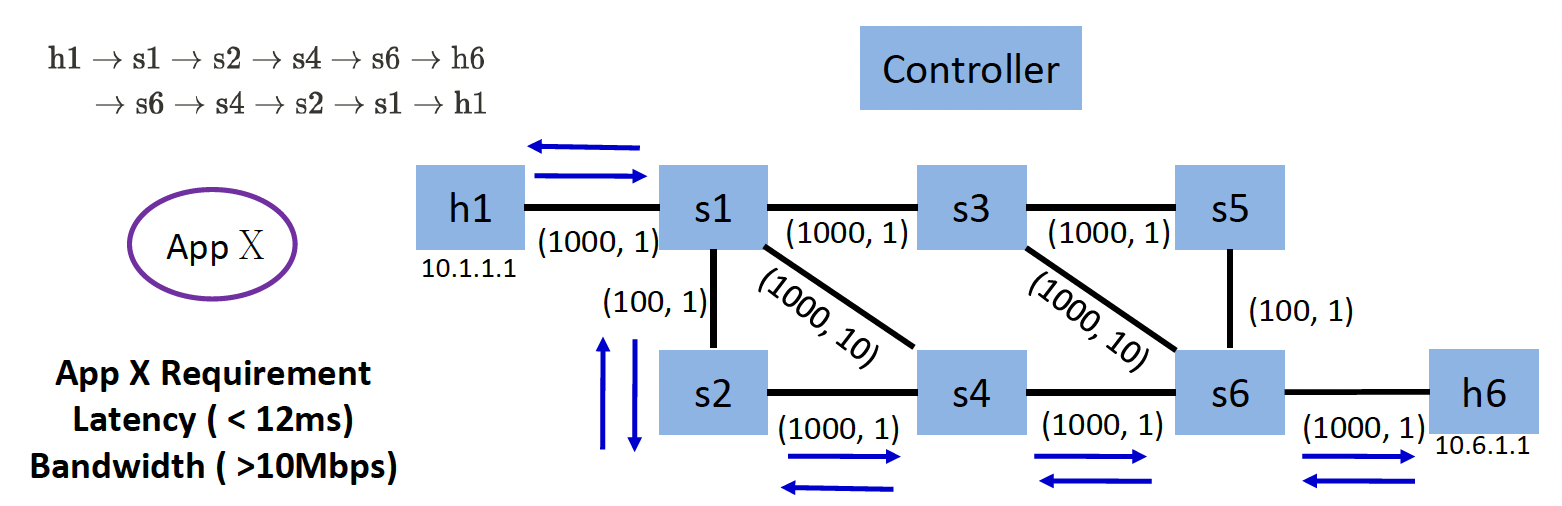
\includegraphics[width=.7\textwidth]{image/week08/e1-0.png}
            	\caption{\footnotesize
            	 Application X의 requirement 를 만족시키는  Routing Path}
            	\vspace{-10pt}
            \end{figure}
            
            해당 path를 따르게 하기위해서 flow table에 다음의 command로 flow를 추가해 주었다.
            \begin{listing}[h!]
            \inputminted[framerule = 1pt,framesep = 2mm , frame = lines, fontsize=\footnotesize]{python}{./code/week08/flow-e1.sh}
            \vspace{-5mm}
            \caption{\footnotesize Extra experiment 1's dpctl flow-add commands}
            \end{listing}
                \vspace{-4mm}
            \begin{figure}[!h]\centering 
            	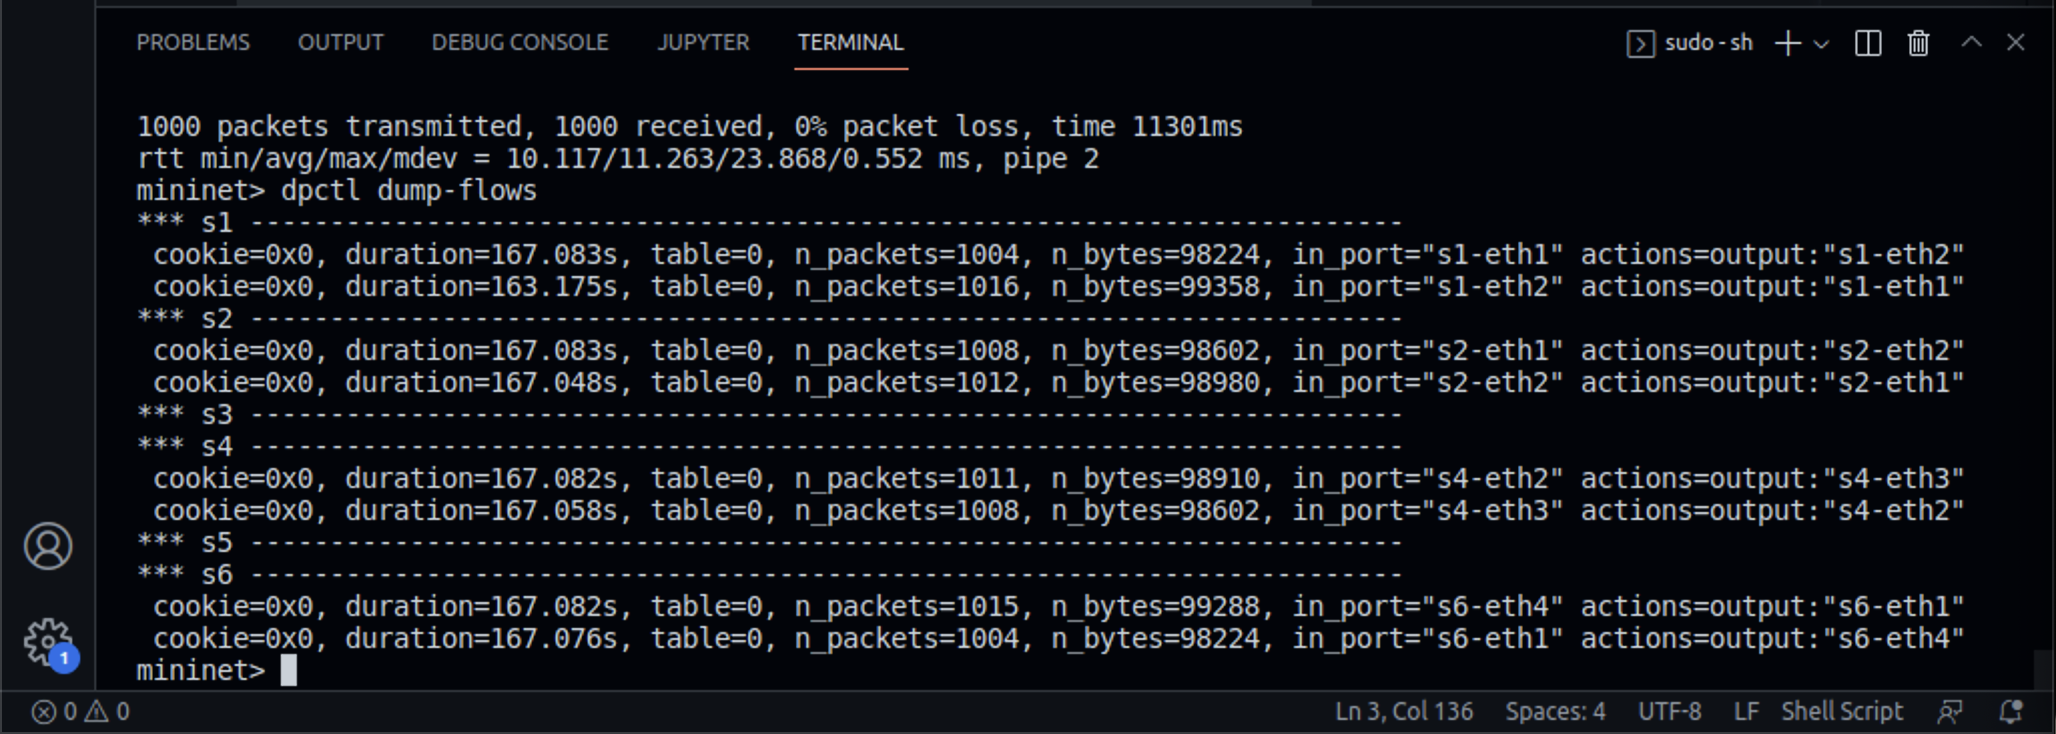
\includegraphics[width=.99\textwidth]{image/week08/e1-1.png}
            	\caption{\footnotesize
            	 Extra experiment 1's flow table}
            	\vspace{-10pt}
            \end{figure}

        \subsubsection*{Ping Table : Latency}
            \vspace{-5mm}
        \begin{equation*}
            \text{Latency} \simeq 0.5 \times \text{Round Trip Time} \quad \Rightarrow 0.5 \times 11.263 = 5.631 ms\ \leq\ 12 ms \to \text{ X application's latency}
        \end{equation*}
            \vspace{-4mm}
        \begin{figure}[!h]\centering 
        	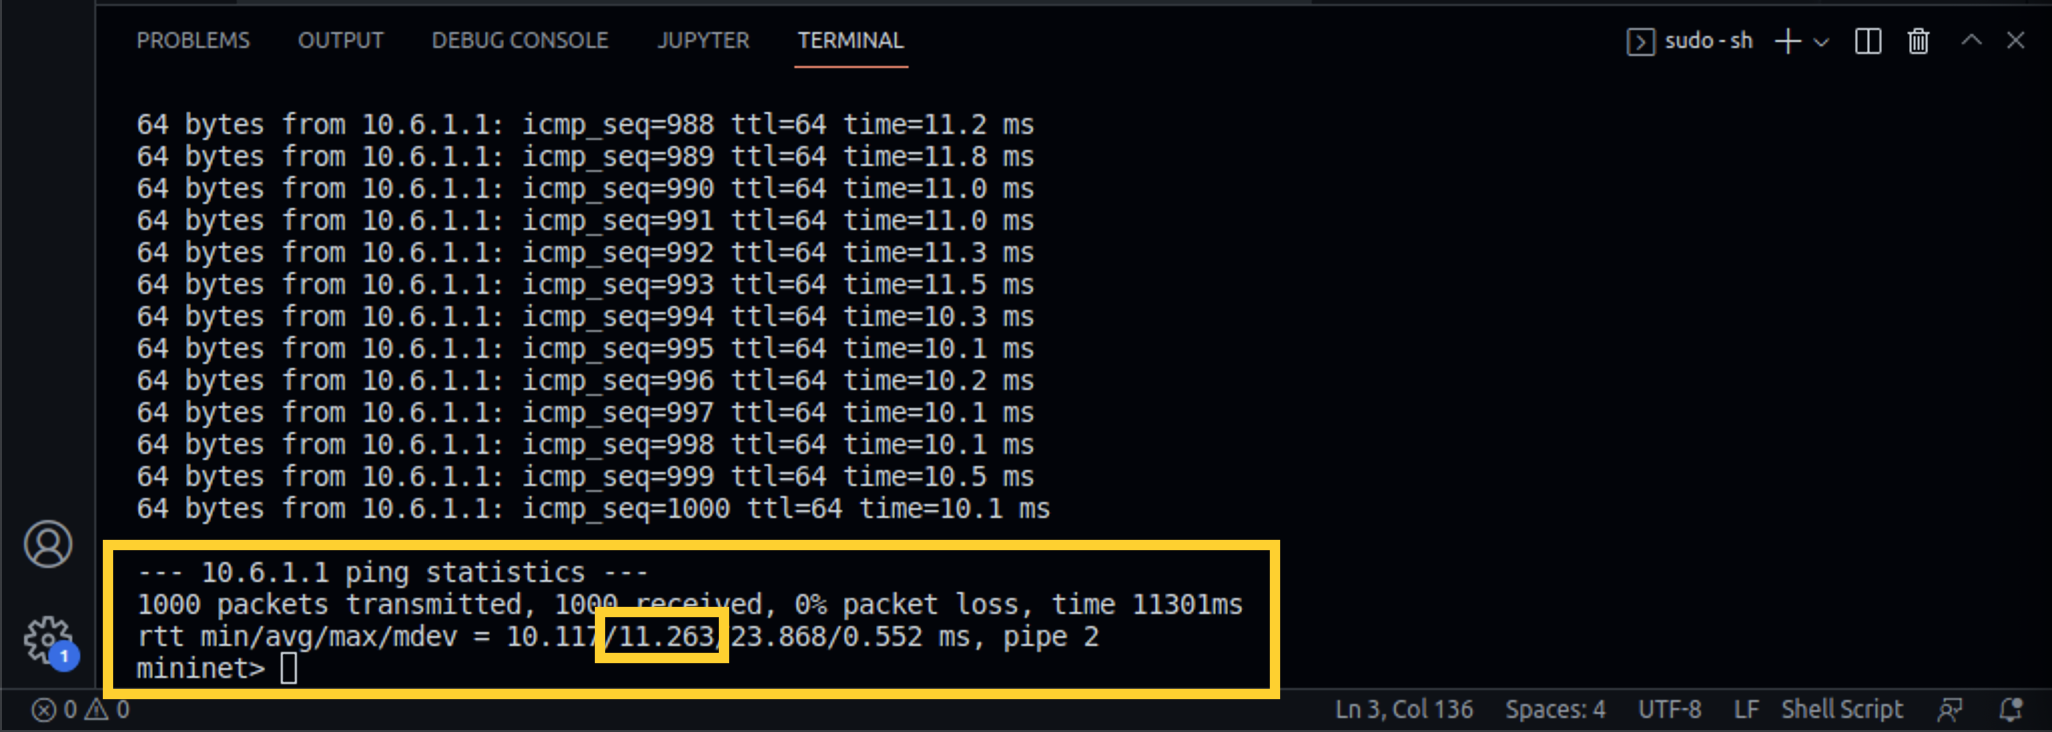
\includegraphics[width=.88\textwidth]{image/week08/e1-2.png}
        	\caption{\footnotesize
        	 Extra experiment 1's pingtest results value of RTT, $11.263\ ms$ average}
        	\vspace{-10pt}
        \end{figure}
            \vspace{-5mm}
        \subsubsection*{ipref Test : Bandwidth}
        대역폭이 88.4 Mbps 와 94.4 Mbps 로  대역폭 기준 인 10 Mbps를 상회하는 결과를 확인할 수 있다. 
        \begin{figure}[!h]\centering 
        	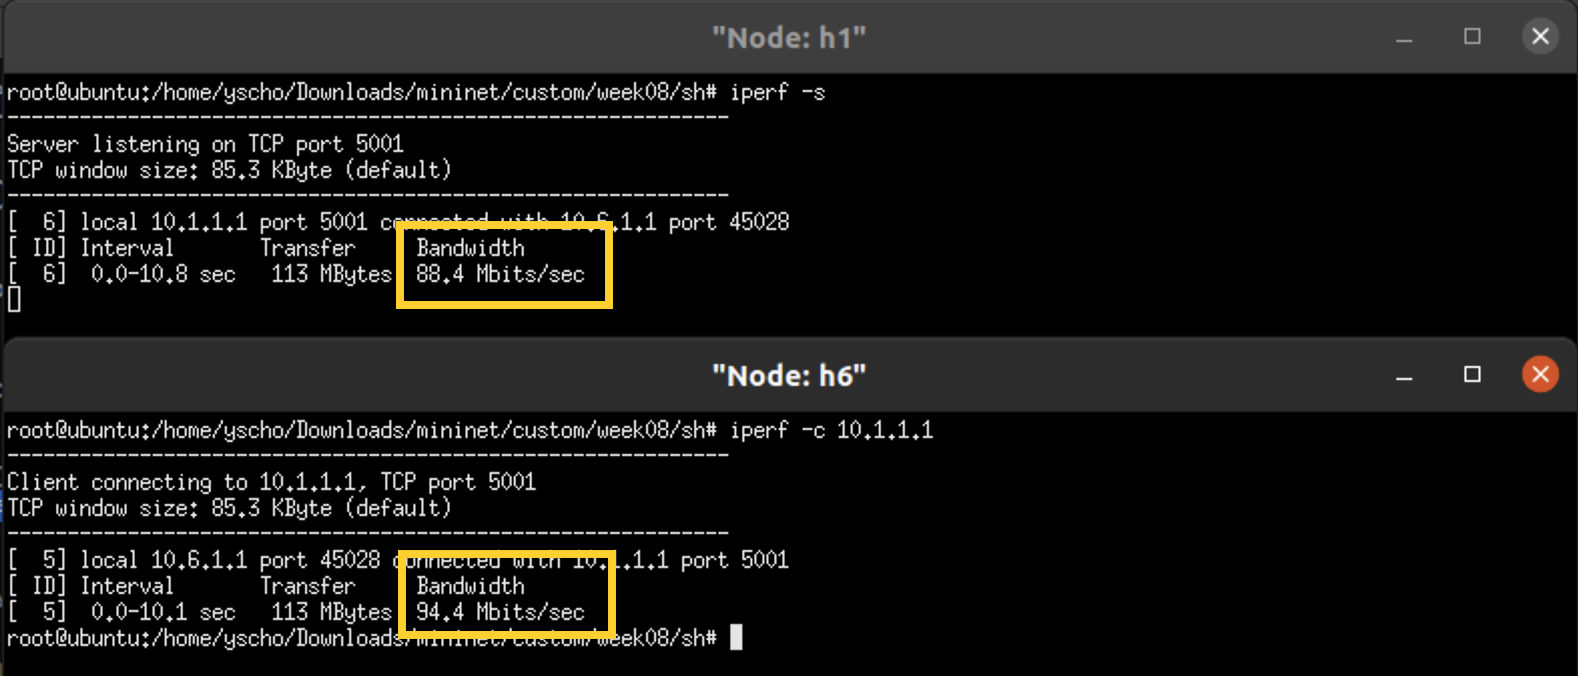
\includegraphics[width=.88\textwidth]{image/week08/e1-3.png}
        	\caption{\footnotesize
        	 Experiment1's the measured bandwidth value of host h1\& h6, 88.4 Mbits/sec 94.4Mbits/sec}
        	\vspace{-10pt}
        \end{figure}
% \clearpage
%---------------------------------------------------------------------------------%